% Double Arrows a la Chef
% Author: Dominik Haumann
\documentclass{article}
\usepackage{tikz}
%\usepackage[svgnames]{xcolor}
%\usepackage{verbatim}
%\usepackage[active,tightpage]{preview}
%\PreviewEnvironment{tikzpicture}
%\setlength{\PreviewBorder}{50pt}%
\usetikzlibrary{backgrounds}


\usetikzlibrary{arrows, decorations.markings}

% for double arrows a la chef
% adapt line thickness and line width, if needed


\begin{document}

\begin{figure}

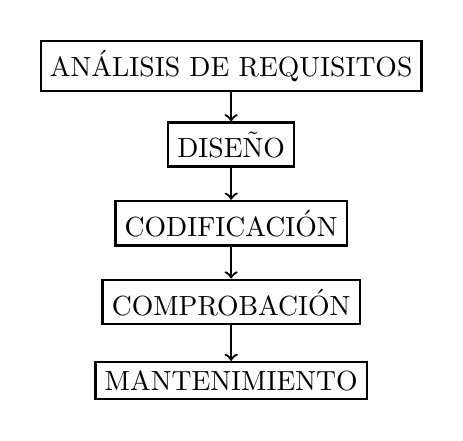
\begin{tikzpicture}[thick, show background rectangle, background rectangle/.style={fill=white}, color=black]
\node[draw,rectangle] (a) {AN\'ALISIS DE REQUISITOS};
\node[draw,rectangle,below of=a] (b) {DISE\~NO};
\node[draw,rectangle,below of=b] (c) {CODIFICACI\'ON};
\node[draw,rectangle,below of=c] (d) {COMPROBACI\'ON};
\node[draw,rectangle,below of=d] (e) {MANTENIMIENTO};

% 1st pass: draw arrows
\draw [->] (a) -- (b);
\draw [->] (b) -- (c);
\draw [->] (c) -- (d);
\draw [->] (d) -- (e);

\end{tikzpicture}
\caption{Fases  en  la  ejecución  de un proyecto  informático: INGENIERÍA DEL SOFTWARE }
\end{figure}

\end{document}